
\section{Neuronale Netze}



Die nachfolgenden Ausführungen und Graphiken zum Schaffen eines grundlegenden Verständnisses des Machine Learnings
basieren im wesentlichen auf dem E-Book "Neural Networks and Deep Learning"\footnote{Michael Nielsen, Neural Networks and Deep Learning.\newline
(http://neuralnetworksanddeeplearning.com/index.html)}.

Im Rahmen des maschinellen Lernens stellen die sogenannten neuronalen Netze einen elementaren Ansatz dar,
der in vielen weiteren Modellen Verwendung findet. Neuronale Netze wie das maschinelle Lernen an sich
stellen eine andere Herangehensweise dar, als die klassischer, deterministischer Algorithmen.

Anstatt dem System eine eindeutige Abfolge von Anweisungen mitzuteilen, um eine konkrete Problemstellung
zu lösen, definiert man ein Modell und konfrontiert dieses mit verschiedenen Beispielen - die Beispiele
sind dabei Tupel aus Eingangsgröße und erwarteter Ausgangsgröße. Die Dimensionen von Eingangs- und Ausgangsgröße
können sich dabei gleichen, müssen es aber nicht. So können als Eingabe Bilder dienen und als
Ausgaben konkrete Klassen, um beispielsweise Hunde von Katzen unterscheiden zu können.

Anstatt nun algorithmisch zu definieren, was einen Hund von einer Katze unterscheidet, überlässt man es dem zuvor
erstellten Modell anhand der gegebenen Eingaben und erwarteten Ausgaben, eigenständig Regeln abzuleiten, um mit
dessen Hilfe auch unbekannte Eingaben klassifizieren zu können.

Dieser Ansatz wird als \textit{Soft Computing} bezeichnet.

\subsection{Perzeptron}

Als elementaren Bestandteil eines neuronalen Netzes dient das sogenannte \textit{Perzeptron} - dieses stellt
die kleinste Einheit eines neuronalen Netztes dar und wird auch als ``künstliches Neuron'' bezeichnet.

Grundsätzlich akzeptiert ein Neuron einen beliebig großen Input bestehend aus Features \textit{x1, x2, ..., xn} und
berechnet daraus ein Ergebnis.

\begin{figure}[h]
    \centering
    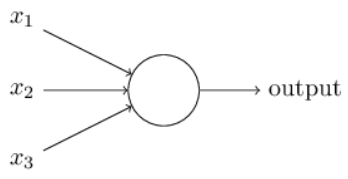
\includegraphics[width=0.5\textwidth]{docu_img_01}
    \caption{Perzeptron}
    \label{fig:perzeptron}
\end{figure}

Im gezeigten Bild ist beispielsweise ein Neuron dargestellt, das drei Inputgrößen akzeptiert und daraus einen Output
produziert. Um den Output zu berechnen werden Gewichte (\textit{engl. weights}) eingeführt. Ob das Neuron 0 oder 1 als
Output liefert, hängt dann davon ab, ob die gewichtete Summe der Eingangsgrößen einen zu definierenden Schwellwert
überschreitet.

Dies kann anhand des nachfolgenden Bilds verdeutlicht werden:

\begin{figure}[h]
    \centering
    \[ output =
      \begin{cases}
        0 \quad \text{if } \sum \omega_i x_i \leqslant \text{ threshold}\\
        1 \quad \text{if } \sum \omega_i x_i > \text{ threshold}
      \end{cases}
    \]
    \caption{Berechnung des Outputs.}
    \label{fig:neuron-three-way}
\end{figure}


Dies ist das grundlegende Modell. Grundsätzlich kann man sich das Perzeptron als einen ``Entscheidungs-Unterstützer''
vorstellen, der eine Entscheidung trifft, in dem er konkrete Fakten mit einem bestimmten Gewicht versieht.

Das gezeigte Modell ist augenscheinlich sehr simpel und noch sehr weit von dem entfernt, was man als ein neuronales
Netz bezeichnen würde. Es ist allerdings ohne Weiteres denkbar, das gezeigte Model komplexer zu gestalten, indem
mehrere Perzeptrons miteinander verknüpft werden, so dass beispielsweise das nachfolgende Netzwerk entstehen könnte:

\begin{figure}[h]
    \centering
    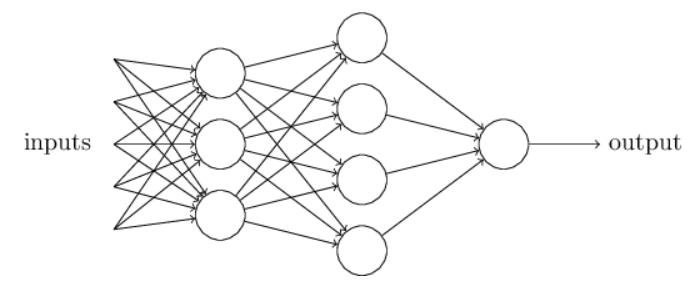
\includegraphics[width=0.5\textwidth]{docu_img_03}
    \caption{Mehrschichtiges neuronales Netz.}
    \label{fig:multi-layer-net}
\end{figure}



In Grafik\textsuperscript{\ref{fig:neuron-three-way}} wurde ein Schwellwert eingeführt, der überschritten werden muss, damit ein Perzeptron
aktiviert wird. Um das Modell zu vereinheitlichen, kann der \textit{Bias} definiert werden, der den
negativen Schwellwert darstellt. Durch diese Maßnahme kann die Aktivierungsfunktion des Perzeptrons dann geschrieben
werden als:

\begin{figure}[h]
    \centering
    \[ output =
          \begin{dcases}
            0 \quad \text{if } \sum \omega \cdot x + b \leq 0 \\
            1 \quad \text{if } \sum \omega \cdot x + b > 0
          \end{dcases}
    \]
    \caption{Berechnung des Outputs bei Verwendung eines Bias.}
    \label{fig:bias-calculation}
\end{figure}

Inhaltlich kann das Bias als ein Maß verstanden werden, aus dem hervorgeht, wie leicht ein Perzeptron aktiviert
werden kann. Nimmt der Bias einen großen Wert an, so kann das Perzeptron einen Wert von 1 annehmen, auch wenn das
Produkt aus den Gewichten und den Eingangsgrößen einen negativen Wert annimmt. Gleiches gilt selbstverständlich auch für
einen kleinen Bias, der zur Folge hat, dass ein Perzeptron träger reagiert.

\subsection{Sigmoid-Neuronen}

Eine Weiterentwicklung des zuvor vorgestellten Modells stellen Sigmoid-Neuronen dar. Diese Weiterentwicklung wird
dann erforderlich, wenn das Anpassen der Gewichte - also letztlich das Lernen - betrachtet wird. Dabei ist das Ziel,
dass eine kleine Anpassung eines Gewichts auch nur eine kleine Änderung des Outputs zur Folge hat. Das zuvor
betrachtete Perzeptron ist lediglich in der Lage 0 oder 1 als Output zu liefern, so dass Änderungen an den Gewichten
keine stetige Änderung des Outputs zur Folge haben, sondern folgenlos bleiben können bis irgendwann ein Sprung von 0
auf 1 oder umgekehrt stattfindet, was wiederum eine große Änderung darstellt.

Die Weiterentwicklung besteht nun in einer Verfeinerung der Aktivierungsfunktion. Anstatt eine Sprungfunktion\textsuperscript{\ref{fig:step-function}} zu
verwenden, die lediglich 0 und 1 als Funktionswert annehmen kann, wird die sogenannte Sigmoid Funktion\textsuperscript{\ref{fig:sigmoid-function}} eingeführt,
die die folgende Form hat:

\begin{figure}[h]
    \centering
    \[ \sigma(z) \equiv
          \frac{1}{1+e^{-z}}
    \]
    \caption{Sigmoid-Funktion.}
    \label{fig:sigmoid}
\end{figure}

Der entscheidende Unterschied kann an den beiden nachfolgenden Grafiken verdeutlicht werden, die jeweils die Kurve
der entsprechenden Funktion darstellen:

\captionsetup[subfigure]{labelformat=empty, labelsep=none}
\begin{figure}[h]
    \centering
    \begin{subfigure}{0.45\textwidth}
		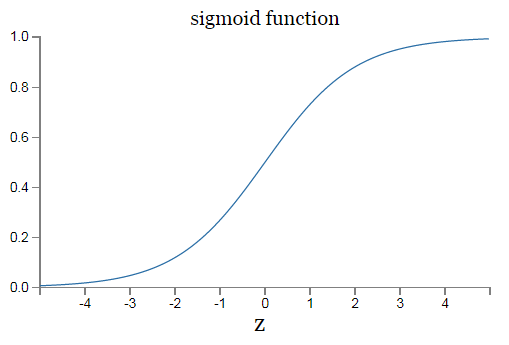
\includegraphics[width=0.9\textwidth]{docu_img_06}
		\caption{\tiny{Sigmoid Funktion.}}
		\label{fig:sigmoid-function}
	\end{subfigure}
    \begin{subfigure}{0.45\textwidth}
		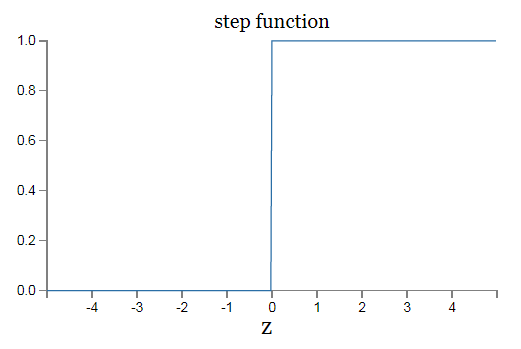
\includegraphics[width=0.9\textwidth]{docu_img_07}
		\caption{\tiny{Step Funktion.}}
		\label{fig:step-function}
	\end{subfigure}

    \caption{Vergleich der Aktivierungsfunktionen \textit{Sigmoid} und \textit{Step-Funktion}}
    \label{fig:activation-functions}
\end{figure}

\subsection{Architektur neuronaler Netze}

Mit diesen Bestandteilen als Ausgangspunkt können nun tatsächlich konkretere Neuronale Netze und deren Architekturen
eingeführt werden. Neuronale Netze bestehen üblicherweise aus mehreren Schichten, den \textit{Layern}. Diese lassen
sich grundsätzlich in drei Kategorien aufteilen: Input, Hidden und Output. Neuronale Netze beinhalten für gewöhnlich
ein Input-Layer und ein Output-Layer sowie dazwischen beliebig viele Hidden-Layer. Die Form der Input- und Output-Layer
ist dabei sehr naheliegend: das Input-Layer hat die gleiche Struktur wie die des Inputs und das Output-Layer hat
entsprechend die gleiche Struktur wie der Output.

Angenommen es sollen Bilder der Größe 28x28 Pixel klassifiziert werden und es gibt 10 mögliche Klassen, dann besteht das
Input-Layer aus 28x28 = 784 Neuronen und das Output-Layer aus 10 Neuronen.

Lediglich der Bereich zwischen Input- und Output-Layer - die Hidden-Layer - lässt sich nicht ohne Weiteres aus dem Input
oder dem Output ableiten. Es gibt lediglich Heuristiken, die beim Design der Hidden-Layer angewandt werden können,
allerdings keine konkreten Regeln, die befolgt werden müssen. Diese Struktur kann anhand des nachfolgenden Bilds
verdeutlicht werden, bei dem - um die Übersichtlichkeit zu wahren - das Input-Layer etwas komprimiert dargestellt wird:

\begin{figure}[h]
    \centering
    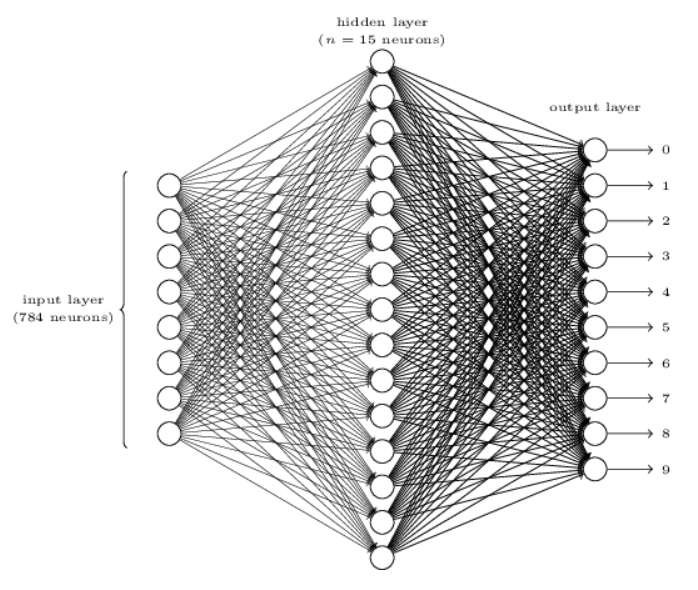
\includegraphics[width=0.9\textwidth]{docu_img_08}
    \caption{Hidden-Layer Darstellung.}
    \label{fig:hidden-layers}
\end{figure}

\subsection{Lernen - Das Anpassen der Gewichte}

Das Lernen stellt den zentralen Ansatz von neuronalen Netzes dar. Eng im Zusammenhang mit dem Lernen steht eine
Kosten-Funktion, die häufig auch als Verlust-Funktion bezeichnet werden kann. Diese stellt letztlich den Fehler zwischen
dem Erwartungswert und dem tatsächlichen Wert, den das neuronale Netz berechnet, dar. Mathematisch betrachtet ist das
grundlegende Prinzip des Lernens diese Funktion zu minimieren, also zu gewährleisten, dass die Abweichungen zwischen
Erwartungswert und tatsächlichem Wert möglichst gering sind. Es sind grundsätzlich viele verschiedene Verlust-Funktionen
denkbar, eine, die jedoch eine breite Verwendeung findet, ist die quadratische Kosten-Funktion - auch als \textit{mean squared
error} (MSE) bezeichnet.

\begin{figure}[h]
    \centering
    \[ C(w, b) \equiv
          \frac{1}{2n}\displaystyle\sum_{x}{\parallel y(x) - a\parallel^2}
    \]
    \caption{Mean Squared Error (MSE).}
    \label{fig:learn-function}
\end{figure}

Dabei beschreiben \textit{w} und \textit{b} die Gewichte bzw. die Bias des neuronalen Netzes und \textit{n} stellt die Anzahl der Trainingsdaten
dar. Der Vektor a beschreibt den Output des Netzes und \textit{\(y(x)\)} stellt den Erwartungswert zu einem Input \textit{x} dar.
Das Ziel besteht nun darin, die Gewichte und Bias so zu manipulieren, dass die gezeigte Funktion einen möglichst kleinen
Wert annimmt.

\subsection{Gradientenabstieg (Gradient Descent)}

Um die soeben eingeführte Kostenfunktion zu minimieren, wird ein Verfahren verwendet, das als Gradientenabstieg (\textit{engl.
gradient descent}) bezeichnet wird. Neben dem hier vorgestellten Verfahren existieren noch viele weitere Methoden, die
zur Lösung dieses Optimierungs- bzw. Minimierungsproblems verwendet werden können.
Zur Veranschaulichung des Problems soll nun eine Funktion zweier Variablen, die minimiert werden soll, betrachtet werden.

\begin{figure}[h]
    \centering
    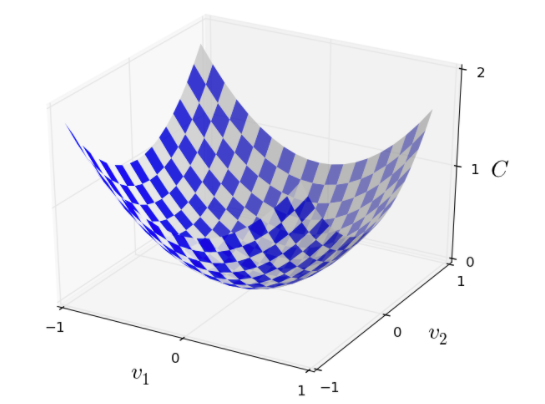
\includegraphics[width=0.9\textwidth]{docu_img_17}
    \caption{Darstellung des Gradientenabstieg bei einer Funktion in Abhängigkeit von zwei Variablen.}
    \label{fig:gradient-decent-3d}
\end{figure}

Dieses Problem könnte selbstverständlich durch Verfahren der Analysis gelöst werden. In der Realität ist die Anzahl der
Variablen jedoch um ein Vielfaches höher, sodass diese Verfahren nicht mehr effizient angewandt werden können.

Zur Visualisierung der grundlegenden Idee des Gradientenabstiegs kann sich ein Ball vorgestellt werden, der sich abwärts
in Richtung eines Tals bewegt. Bewegt man den Ball etwas in Richtung \textit{v1} und etwas in Richtung \textit{v2}
so gilt für den Funktionswert \textit{C}:

\begin{figure}[h]
    \centering
    \[ \Delta C \approx
          \frac{\delta C}{\delta v_1} \Delta v_1 + \frac{\delta C}{\delta v_2} \Delta v_2
    \]
    \caption{Veränderung des Funktionswerts.}
    \label{fig:gradient-decent-definition}
\end{figure}

Der Gradient wird dann folgendermaßen definiert:

\begin{figure}[h]
    \centering
    \[ \nabla C \equiv
        (\frac{\delta C}{\delta v_1},\frac{\delta C}{\delta v_2})^T
    \]
    \caption{Definition des Gradienten}
    \label{fig:gradient-decent-definition-2}
\end{figure}

Durch die Verwendung dieses mathematischen Objekts kann die vorherige Gleichung\textsuperscript{\ref{fig:gradient-decent-definition}} formuliert werden als:

\begin{figure}[h]
    \centering
    \[ \delta C \approx
        \nabla C \cdot \delta v
    \]
    \caption{Veränderung des Funktionswerts durch Gradienten ausgedrückt}
    \label{fig:gradient-decent-definition-3}
\end{figure}

Wird die Veränderung der Variablen (Gewichte) nun so gewählt, dass sie dem Inversen des Gradienten multipliziert mit
einem kleinen, positiven Faktor (Lernrate) entspricht, kann sichergestellt, dass sich dem Minimum der Funktion
genähert wird.

Dieses Vorgehen wird mehrfach - genau genommen für jeden Durchlauf der Trainingsdaten - wiederholt, bis die dadurch erzielte Näherung den
Ansprüchen an die Genauigkeit genügt.

\subsection{Convolutional Networks}

Insbesondere bei der Klassifizierung von Bildern hat sich eine bestimmte Art von neuronalen Netzen als besonders passend
herausgestellt - dabei handelt es sich um die \textit{Convolutional Networks}. Diese zeichnen sich dadurch aus,
dass sie auch die räumliche Struktur der Bilder berücksichtigen: Während herkömmliche \textit{fully connected} neuronale Netze
sämtliche Pixel gleich behandeln würden, unabhängig davon, ob sie beispielsweise benachbart sind oder nicht, betrachten
Convolutional Networks immer nacheinander konkrete Abschnitte eines Bilds, um Strukturen zwischen benachbarten Pixeln
erkennen und somit verarbeiten zu können.
Dabei liegen den Convolutional Networks im Wesentlichen drei Ideen zugrunde:

\begin{enumerate}
    \item{Local receptive field}
    \item{Shared weights}
    \item{Pooling}
\end{enumerate}

\subsubsection{Wesentliche Konzepte von Convolutional Networks}

Diese Bestandteile sollen nun nachfolgend einzeln genauer betrachtet werden.

\textnormal{\paragraph{Local receptive field}}

Für das Verständnis des lokalen rezeptiven Felds (\textit{local receptive field}) empfiehlt es sich, die Input-Neuronen des
Convolutional Networks nicht als vertikale Linie von Neuronen, sondern vielmehr in den Dimensionen des Bildes, das von
dem Netzwerk betrachtet werden soll, zu visualisieren. Werden beispielsweise Bilder der Größe 28x28 Pixel betrachtet
entspräche das dem nachfolgenden Input-Layer:

\begin{figure}[h]
    \centering
    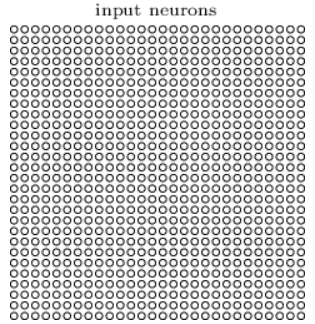
\includegraphics[width=0.5\textwidth]{docu_img_10}
    \caption{Feld von Inputneuronen.}
    \label{fig:field-of-neurons}
\end{figure}

Im Unterschied zu \textit{herkömmlichen} neuronalen Netzen, bei denen üblicherweise alle Input-Neuronen mit allen Neuronen des
nachfolgenden Hidden-Layers verbunden werden, besteht die Besonderheit nun darin, dass jedes Neuron des Hidden-Layers
mit einem kleinen Bereich des Inputs verbunden wird. Dieses Vorgehen kann anhand des folgenden Bildes veranschaulicht
werden:

\begin{figure}[h]
    \centering
    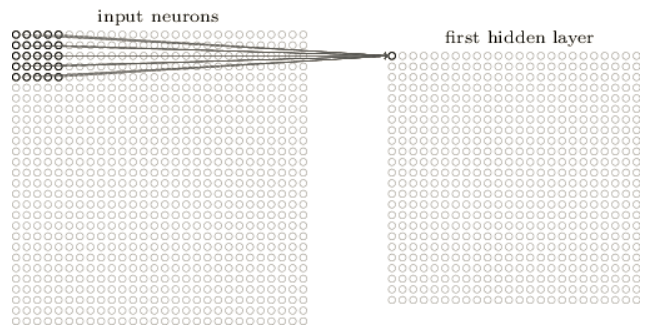
\includegraphics[width=0.9\textwidth]{docu_img_11}
    \caption{Convolution-Prozess, Schritt 1.}
    \label{fig:convolution-process-1}
\end{figure}

Dieses lokale rezeptive Feld wird dann gemäß der Konfiguration über das Input-Bild \textit{bewegt}, so dass alle Input-Neuronen
besucht werden. Demnach sähe der zweite Schritt - unter der Annahme, dass das Feld immer um ein Pixel verschoben wird -
folgendermaßen aus:

\begin{figure}[h]
    \centering
    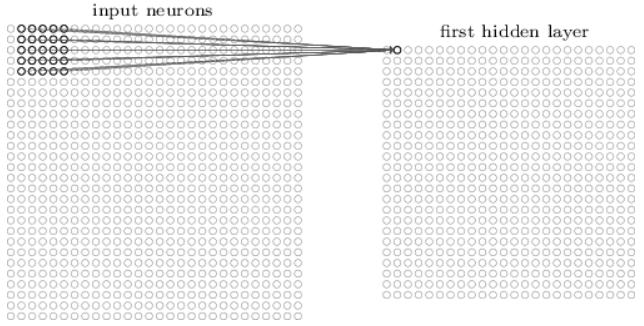
\includegraphics[width=0.9\textwidth]{docu_img_12}
    \caption{Convolution-Prozess, Schritt 2.}
    \label{fig:convolution-process-2}
\end{figure}

Auf diese Art und Weise entsteht das erste Hidden-Layer dessen Größe selbstverständlich etwas kleiner ist, als die Größe
des Input-Layers. Geht man von einem Input-Bild der Größe 28x28 Pixel und einem lokalen rezeptiven Feld der Größe 5x5
Pixel aus, so folgt daraus ein erstes Hidden-Layer der Größe 24x24 Pixel.

\textnormal{\paragraph{Shared weights}}

Jedes Neuron des Hidden-Layers verfügt wie üblich über einen Bias und - im Falle eines lokalen rezeptiven Felds der
Größe 5x5 Pixel - über 5x5 Gewichte. Die Besonderheit besteht nun darin, dass diese Gewichte und Bias für ALLE Neuronen
des Hidden-Layers gleich gelten. Inhaltlich hat dies zur Folge, dass ein konkretes Hidden-Layer genau eine konkrete
\textit{Auffälligkeit} extrahiert. Solch eine konkrete \textit{Auffälligkeit} könnte beispielsweise eine vertikale oder horizontale
Linie sein, die durch die Verwendung des lokalen rezeptiven Felds, das sich über das Bild bewegt, an beliebigen
Positionen aufgespürt werden kann. Üblicherweise reicht es nicht aus, nur eine \textit{Auffälligkeit} aufzuspüren. Aus diesem
Grund besteht ein einziges Layer häufig aus mehreren parallelen feature maps (TODO: Begriff einführen)).

So könnte ein einziges Hidden-Layer beispielsweise die nachfolgende Form haben, durch das dann drei verschiedene
Auffälligkeiten extrahiert werden würden:

\begin{figure}[h]
    \centering
    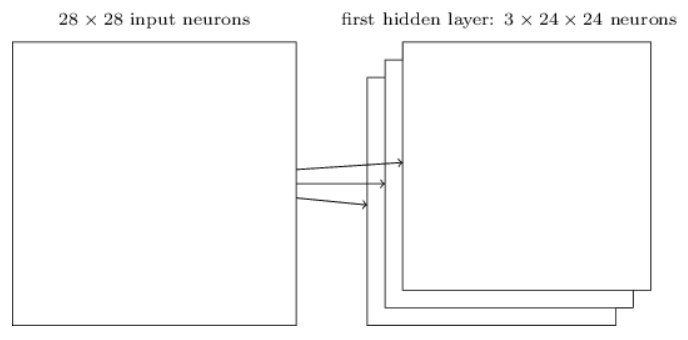
\includegraphics[width=0.9\textwidth]{docu_img_13}
    \caption{Drei Filterschichten.}
    \label{fig:filter-layers}
\end{figure}

Ein weiterer wesentlicher Vorteil bei der Verwendung von \textit{shared weights} besteht darin, dass die Anzahl der zu
trainierenden Variablen um ein Vielfaches verringert wird, wodurch ein schnelleres Lernen ermöglicht werden kann.
Eine einzige feature map (TODO) würde bei den bisher betrachteten Dimensionen durch 5x5 = 25 Gewichte und einen Bias,
also insgesamt 26 Parameter definiert werden. Selbst wenn ein Hidden-Layer aus 20 features maps bestünde, so würde dies
im Ergebnis zu \textit{nur} 20x26 = 520 Parametern führen.
Wird ein fully connected Layer bestehend aus 30 Neuronen und das gleiche Input-Layer wie zuvor betrachtet, so folgt
daraus, dass insgesamt (28 x 28) x 30 + 30 = 23550 Parameter in jedem Schritt des Lernens angepasst werden müssen.

\textnormal{\paragraph{Pooling}}

Die zuvor vorgestellten Layer, die durch die Verwendung des lokalen rezeptiven Felds und gemeinsam geteilter Gewichte
enstehen, werden gemeinhin als \textit{convolutional} Layer bezeichnet. Von diesen kann ein weiterer wesentlicher Bestandteil
von convolutional networks abgegrenzt werden - die sogenannten \textit{pooling} Layer. Diese Art von Layer folgt für
gewöhnlich auf die zuvor vorgestellten \textit{convolutional} Layer und hat zur Aufgabe, die dadurch gewonnenen Informationen
zu vereinfachen.
Das grundsätzliche Vorgehen kann durchaus mit dem des convolutional Layers verglichen werden - auch bei den pooling
Layers kommt ein Feld zum Einsatz, dass sich über das Ergebnis des vorherigen Schrittes bewegt. Es könnte sich
beispielsweise um ein Feld der Größe 2x2 handeln. Dieses würde somit immer 4 Neuronen betrachten und - im Falle des
sogenannten max-poolings (einer konkreten Ausprägung des Poolings) - das größte von ihnen auswählen.

Bildlich kann dies auf die folgende Art und Weise veranschaulicht werden:

\begin{figure}[h]
    \centering
    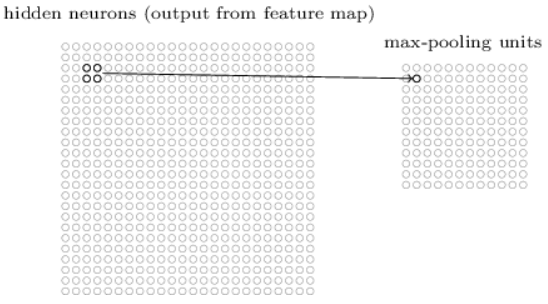
\includegraphics[width=0.9\textwidth]{docu_img_14}
    \caption{Maxpooling Prozess.}
    \label{fig:max-pooling}
\end{figure}

Dadurch, dass vier Neuronen auf ein Neuron projeziert werden, verringert sich die Größe bei diesem konkreten Beispiel
von 24x24 auf 12x12. Dieses Vorgehen wird selbstverständlich auf alle feature maps des vorherigen convolutional Layers
angewendet, so dass das folgende Ergebnis entsteht.

\begin{figure}[h]
    \centering
    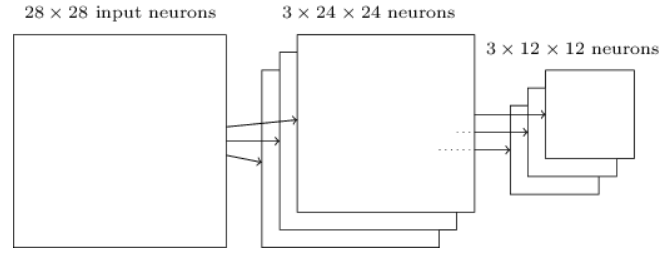
\includegraphics[width=0.9\textwidth]{docu_img_15}
    \caption{Convolution Prozess.}
    \label{fig:convolution-process}
\end{figure}

\subsubsection{Beispielhaftes Convolutional Network}

Nachdem die wesentlichen Bestandteilen eines convolutional Netzes vorgestellt worden sind, können diese nun miteinander
verknüpft werden, um die Architektur eines exemplarischen Netzes zu veranschaulichen. Wie auch bei \textit{normalen} neuronalen
Netzen orientieren sich Input- und Output-Layer an der Struktur des Inputs bzw. Outputs. Dazwischen befinden sich
abwechselnd convolutional und pooling Layer, die grundsätzlich beliebig oft hintereinander geschaltet werden können.
Demnach sähe ein sehr simples convolutional Netzwerk beispielsweise folgendermaßen aus:

\begin{figure}[h]
    \centering
    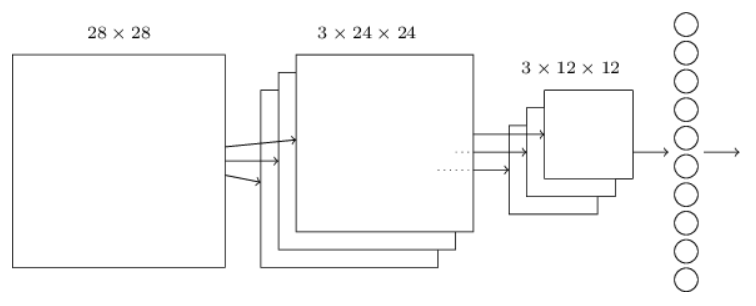
\includegraphics[width=0.9\textwidth]{docu_img_16}
    \caption{Vollständiges \textit{Convolutional Network mit Klassifizierungs-Ausgabe.}}
    \label{fig:convoultional-newtork}
\end{figure}
